\documentclass{article}
\usepackage{tikz}
\usepackage{xcolor}
\begin{document}
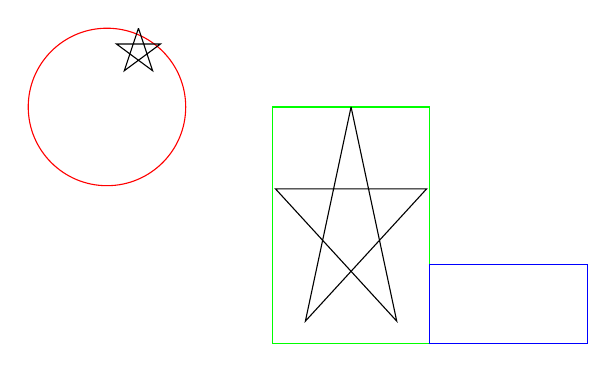
\begin{tikzpicture}
\definecolor{myColor}{RGB}{255,0,0}
\draw[myColor] (0.9,18) circle (1cm);
\definecolor{myColor}{RGB}{0,255,0}
\draw[myColor] (3,18) rectangle (5,15);
\definecolor{myColor}{RGB}{0,0,255}
\draw[myColor] (5,16) rectangle (7,15);
\definecolor{myColor}{RGB}{0,0,0}
\draw[myColor] (1.3,19) -- (1.48,18.46) -- (1.02,18.8) -- (1.58,18.8) -- (1.12,18.46) -- (1.3,19);
\definecolor{myColor}{RGB}{0,0,0}
\draw[myColor] (4,18) -- (4.58,15.28) -- (3.04,16.96) -- (4.96,16.96) -- (3.42,15.28) -- (4,18);
\end{tikzpicture}
\end{document}
